\documentclass[10pt,twopage]{acmsiggraph}

\usepackage{fancyheadings} % we need page numbers...
\usepackage{times}
\usepackage{graphicx}
\usepackage{hyperref}
\usepackage{latexsym}
\usepackage{hyperref}
\usepackage{amsmath}
\usepackage{amssymb}
\usepackage{amsthm}
\usepackage{amsfonts}
\usepackage{epsfig}


% allow for many figures and tables on one page
\renewcommand{\topfraction}{1.0} % all floats ok
\setcounter{totalnumber}{10}     % #floats = 10
\renewcommand{\textfraction}{0.0} % no text ok
\renewcommand{\dbltopfraction}{0.4}


% override page numbering conventions of the acm style
\pagestyle{fancyplain}
\lhead[\name]{}		% author name on the left for even pages
\rhead[]{\name}		% and on the right for odd pages
\setcounter{page}{1}	% I need to change this line for the proceedings


%%%%%%%%%%%
%
% Do not change anything above this line!!!
%
%%%%%%%%%%%



\begin{document}
\newcommand\result{0.01\%}
\newcommand\iteration{50000 }

%%%%%%%%%%%%%%%%%%%%%%%%%%%%%%%%%%%%%%%%%%%%%%%%%%%%%%%%%%%%%%%%%%%%%%%%
%%%%%%%%%%%%%%%%%%%%%%%%%%%%%%%%%%%%%%%%%%%%%%%%%%%%%%%%%%%%%%%%%%%%%%%%
%
% Title and author(s)
%
%%%%%%%%%%%%%%%%%%%%%%%%%%%%%%%%%%%%%%%%%%%%%%%%%%%%%%%%%%%%%%%%%%%%%%%%
%%%%%%%%%%%%%%%%%%%%%%%%%%%%%%%%%%%%%%%%%%%%%%%%%%%%%%%%%%%%%%%%%%%%%%%%

\title{Poisson Image Solver}

\newcommand\name{C. Albert Thompson}

\author{\name\\
\\
Department of Computer Science\\
The University of British Columbia}

\maketitle

%%%%%%%%%%%%%%%%%%%%%%%%%%%%%%%%%%%%%%%%%%%%%%%%%%%%%%%%%%%%%%%%%%%%%%%%
%%%%%%%%%%%%%%%%%%%%%%%%%%%%%%%%%%%%%%%%%%%%%%%%%%%%%%%%%%%%%%%%%%%%%%%%
%
% Abstract
%
%%%%%%%%%%%%%%%%%%%%%%%%%%%%%%%%%%%%%%%%%%%%%%%%%%%%%%%%%%%%%%%%%%%%%%%%
%%%%%%%%%%%%%%%%%%%%%%%%%%%%%%%%%%%%%%%%%%%%%%%%%%%%%%%%%%%%%%%%%%%%%%%%

\begin{abstract}
This paper presents the Jacobi method to solve Poisson's equation and regenerate images from the divergence of an original image. There has been a lot of related work that implement Poisson solvers, which explains the steps necessary to generate an image using a linear solver. Poisson's equation can be simplified to be solved by a linear equation, and this paper uses the Jacobi method approach. The program calculates divergence of the original image and the Jacobi method is able to approximate an image similar to the original.  Regenerated images use an iteration count of \iteration. The project also implements a basic watermark feature that adds watermarks to an image. Future work of the project can further implement different types of image manipulation, such as copy paste, image restoration and other linear solvers. This paper demonstrates one approach to solve Poisson's equation for image regeneration.
\end{abstract}

%%%%%%%%%%%%%%%%%%%%%%%%%%%%%%%%%%%%%%%%%%%%%%%%%%%%%%%%%%%%%%%%%%%%%%%%
%%%%%%%%%%%%%%%%%%%%%%%%%%%%%%%%%%%%%%%%%%%%%%%%%%%%%%%%%%%%%%%%%%%%%%%%
%
% Introduction
%
%%%%%%%%%%%%%%%%%%%%%%%%%%%%%%%%%%%%%%%%%%%%%%%%%%%%%%%%%%%%%%%%%%%%%%%%
%%%%%%%%%%%%%%%%%%%%%%%%%%%%%%%%%%%%%%%%%%%%%%%%%%%%%%%%%%%%%%%%%%%%%%%%

\section{Introduction}
\label{Intro}
 

The goal of this project is to understand how image reconstruction is done using Poisson's equation, and then implement a simple reconstruction algorithm on an image.

Restoring dated or printed images becomes more prominent as older images become affected by time. Using chemicals to print photos is a good way to have them last a long time. A long time is not enough, photos have been around for two hundred years, and photos will inevitably get damaged either by light, or any other of the many ways to damage printed photos. Figure \ref{family} shows a photo that is about twenty years old and it is facing noticeable damage \ref{family}. As you can see here are vertical lines running across the photo and there is noticeable fading of the whole photo. 

Restoration of images has been around for many years and early work used Fourier-transformation to restore images \cite{richardson72}. His work was later build upon by future authors such as \cite{Bertalmio}, and \cite{Perez}. They were able to use the old well known Poisson's equation to solve for images and repair damage or images with missing pieces. These authors used Poisson's equation to restore images in more discrete methods.

Our project takes a further look at solving Poisson's equation to regenerate images, and leaves restoration of images for future work. Initial investigation of related work shows that most authors do manipulations on gradient fields and then restore the image using  divergence.  The reason Poisson's equation is so useful is that it is a partial differential equation, and allows computation an image from it's divergence. 

When Poisson's equation is setup properly a linear solver may be used to retrieve an image from the divergence. The Jacobi method is the linear solver we use to solve Poisson's equation. Our implementation of the Jacobi method reconstructs an image in \iteration number of iterations. With these initial results show the importance of linear solvers and Poisson's equation.

This paper shows how to calculate the gradient of an image. The first step is to change the image into a scalar function. The scalar function is used to calculate gradient field of an image. The gradient of the image allows us to make minor changes to an image, and even make estimations where images contain artifacts. After the gradient manipulations occur the divergence of the image is restored using Poisson's equation. 

\begin{figure}
\centering
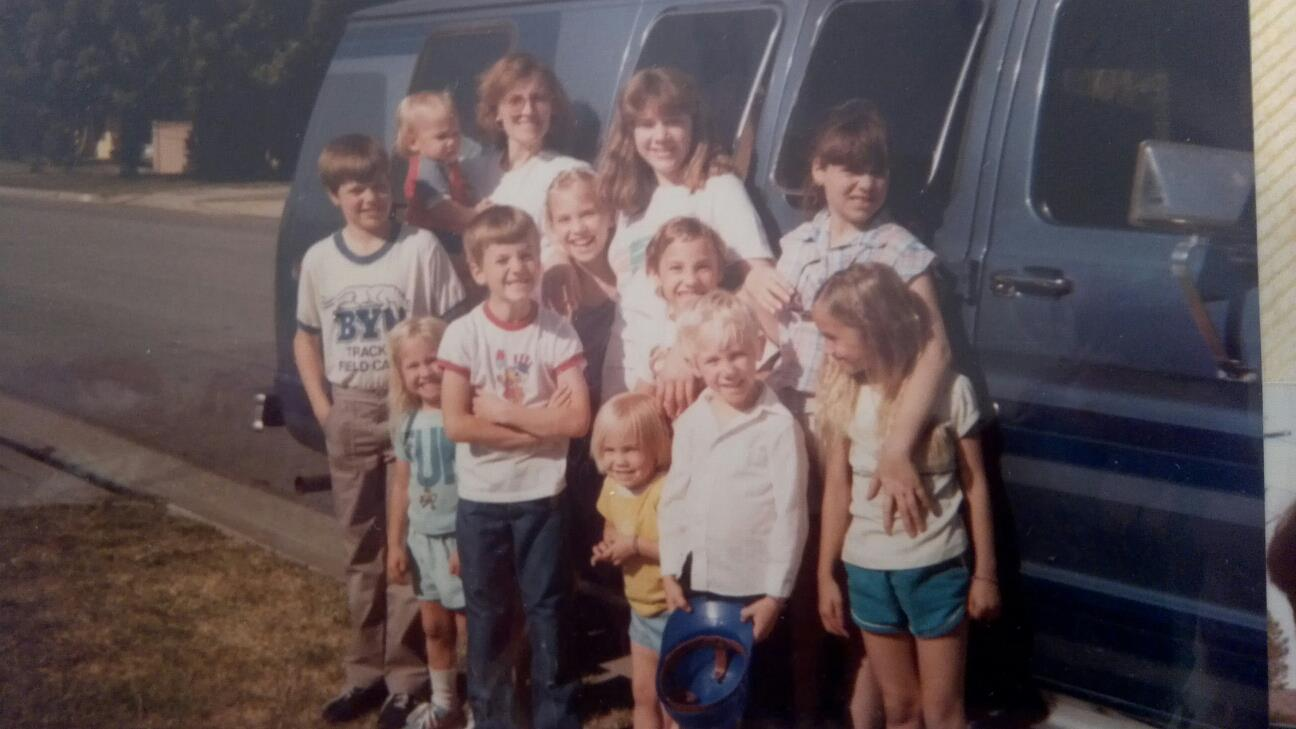
\includegraphics[width=.44\textwidth]{fig/family.jpg}
\caption{An old picture of C. Albert's family.}
\label{family}
\end{figure}


This process shows how to add images together to get a completely new image. This paper shows the results of using a Jacobi solver to regenerate an image from its divergence. We manipulate an image divergence by merging two images together to add a simple watermark to an image. The results of this paper are promising and give us many paths to take to improve our methods.

The goal of this project is to understand how image reconstruction is done using Poisson's equation, and then implement a simple algorithm to regenerate an image from the divergence a vector. 

The rest of paper is outlined as follows. Section 2 discusses current research in Poisson image restoration. Section 3 is dedicated to introducing explaining Poisson's equation, gradients and a way to solve Poisson's equation for image restoration. Section 4  explains artifacts and proposes methods to remove them. In section 5 talks about the future work. Section 6 is the conclusion.


\section{Related work}
\label{relatedWork}
Using Poisson's equation to reconstruct and repair images is a popular method, because it allows images to be transformed into vectors and manipulated. The resulting vectors can be solved with Poisson's equation retrieve a smooth image. An initial analysis shows that recently \cite{Bertalmio} Poisson's equation has been used to do image reconstruction. The current work includes many different ways of doing image reconstruction. One field looks at taking current images that are damaged or missing parts and using gradient and Poisson to reconstruct the image. Another area looks at dragging and dropping images on top of each other then treat the resulting image as a damaged image and do the repair using Poisson.

Bertalmio et al. introduces their paper by making a goal that they want to repair damaged photos. These photos may have inpainting, meaning adding text on top of a picture. The authors also include photos that are damaged or missing parts of the image. Their contribution is different from other approaches as they do not require user input to define the texture of the spot being restored. They create a tool that uses partial differential equations and a mask to determine the area to be filled in and reconstructed. Once they fill in the area they use a smoothness function to improve the image. \cite{Bertalmio} made a major contribution by allowing restoration of images to be done automatically.

Image completion is bad in many cases because it lacks gradient of an image and thus cannot fill in missing parts of an image without having significant artifacts. To overcome this problem \cite{Shen} introduces three steps in the process. First a gradient-patch is used to make up gradient that should be in the image. Then second gradient-patches use an update measure to find the distance between the source patch and a target in the gradient domain. Last the image is completed using Poisson's equation on the gradient map generated by the tool. 

Image reconstruction has also been extended to restoring documents that have folds and other geometric distortions. \cite{sun} combines 3D imaging with Poisson image restoration. Two initial challenges present themselves in using 3D images first shading, and second geometric correction. The paper first solves this problem using previous work on the related subjects. \cite{Ballester} Once the image has been restored to its 2D format then they solve Poisson equation and restore the image. This is work is useful for restoring fragile documents without touching them.

Mixing images is a difficult task to accomplish because the every image has a different gradient field. The gradients are important because it is what allows an image to seemingly mesh together. \cite{Perez} offered a solution to fix the problem of images not being able to be place together. They do this without causing major clashing of the two images. They mix the gradients of the images together by weaving the two images into one another. They also made a contribution selecting only part of an image that one might want to reconstruct and then running Poisson's partial differential equation on that section, this was accomplished by using a mask. These tools improved the field of image drag and drop.

Drag and drop images as previously mentioned simply selected an image and dropped it onto the destination image. By doing this the destination image may contain undesired artifacts. \cite{ddp} offers a way to avoid having these artifacts. They make automatic edits to the image being dropped into a destination image. This method looks at when the boundary of the image that is being dropped is different than the gradient of the destination image. They change the boundary and make the image fit nicer into the destination image.

\section{Poisson}

The related work gives insight on using Poisson's equation to solve for an image. Understanding Poisson's equation is necessary to reconstruction an image. The next step is to retrieve a gradient field of an image. With the gradients a linear method is used to solve Poisson's equation restore an image from the divergence from the gradient field. This project shows the setup Poisson's equation, manipulate an image and restore the image from a gradient field.

\subsection{Poisson Equation}
\label{Poisson}

\begin{figure}
\centering
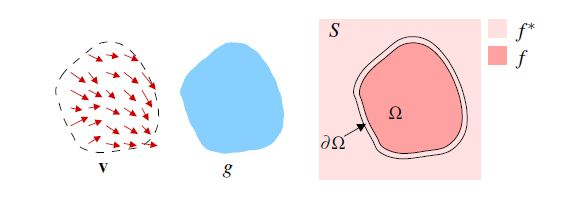
\includegraphics[width=.44\textwidth]{fig/notations.jpg}
\caption{{\bf Guided interpolation notations}. Unknown function $f$ interpolates in domain \ensuremath{\Delta} the destination function $f^*$, under guidance of vector field {\bf v}, which is an example gradient field of a source function $g$}
\label{notations}
\end{figure}

Figure \ref{notations} taken from \cite{Perez} illustrates notations used in applying Poisson's equation to our image editing problem. S is a domain  for the function $f$ which is a closed subset of  \ensuremath{\mathbb{R}^2}. \ensuremath{\Omega} is a closed subset of S with the function $f^*$. {\bf v} is the vector field of image  \ensuremath{\Omega}. 

Poisson's equation is a partial differential equation that is expressed as follows:
\begin{equation} 
\ensuremath{\Delta \varphi = f}
\end{equation}
\ensuremath{\Delta} is the Laplace operator, which is a differential operator. The \ensuremath{ \varphi(x,y) } and $ f(x,y) $ are functions, in $\mathbb{R}^2$ domain. In this project Poisson's equation is used to regenerate 2D images. 

%We represent the Laplacian operator as \ensuremath{\nabla^2}. This representation is to show that we are working with images in 2D space.





Poisson's equation is used to solve the \ensuremath{\Omega} to get an image $f$. This can be accomplished using satisfying the associated Euler-Lagrange equation \ensuremath{\Delta f = 0} over \ensuremath{\Omega}, \ensuremath{\Delta} in our equation is represented as \ensuremath{\frac{\delta^2}{\delta x^2} + \frac{\delta^2}{\delta y^2}}. We now transform this problem into a minimization problem to solve the image $f$.

For the minimization problem we define it as the simplest interpolant $f$ of $f^*$ over \ensuremath{\Omega} and represent it by the following equation:

\begin{equation}
\ensuremath{{\bf min}_f \iint_{\Omega}{|\Delta f|^2}}
\label{min}
\end{equation}

Include the vector field {\bf v} to the minimization equation (\ref{min}). We now apply the directly to the vector field {\bf v}.:

\begin{equation}
{\bf min}_f \iint_{\Omega}{|\Delta f - {\bf v}|^2}
\label{minPoisson}
\end{equation}
there problem has a unique solution with Dirichlet boundary conditions and is expressed:

\begin{equation}
\Delta f = div {\bf v} \mbox{ over \ensuremath{\Omega}}
\label{poissonEqn}
\end{equation}
We use this equation for each of the three colors in the RGB space to solve for the colored image $f$. All the results in this paper are reported with solving equation (\ref{minPoisson}) and each color red blue and green of an image is independently solved. 

\subsection{Gradient and Divergence}

To get a gradient field an image must be represented as a scalar function. The divergence in equation \ref{poissonEqn} is derived from the gradient field. The following preliminary steps  are necessary to setup Poisson's equation 1) represent the image as a scalar, 2) have an equation to calculate the gradient, 3) take care of boundary conditions, 4) calculate the divergence and 5) normalize results to represent as an image.

In order to calculate a gradient we need a scalar function.
\begin{equation}
\ensuremath{f(x,y)}
\label{scalar}
\end{equation}
This scalar function can be used to take the partial derivative of $x$ and $y$ to get a gradient field. The gradient field is the rate of change in the $x$ and $y$ direction and is represented by the following equation:

\begin{equation}
\label{gradient}
\ensuremath{\nabla f = ( \frac{\delta f}{\delta x} , \frac{\delta f}{\delta y} )}
\end{equation}

To get a gradient field an image be represented as a scalar function. An easy way to represent the image as a scalar is to represent each pixel as a red green blue (RGB) value. This project uses that method to represent an image $f$ with the variables $x$, and $y$ the x, y coordinates of the pixel in the image. The return value of function $f$ is an integer representation of the RGB value for each pair $(x,y)$. This is how we represent our image as a scalar function.

\begin{figure}
\centering
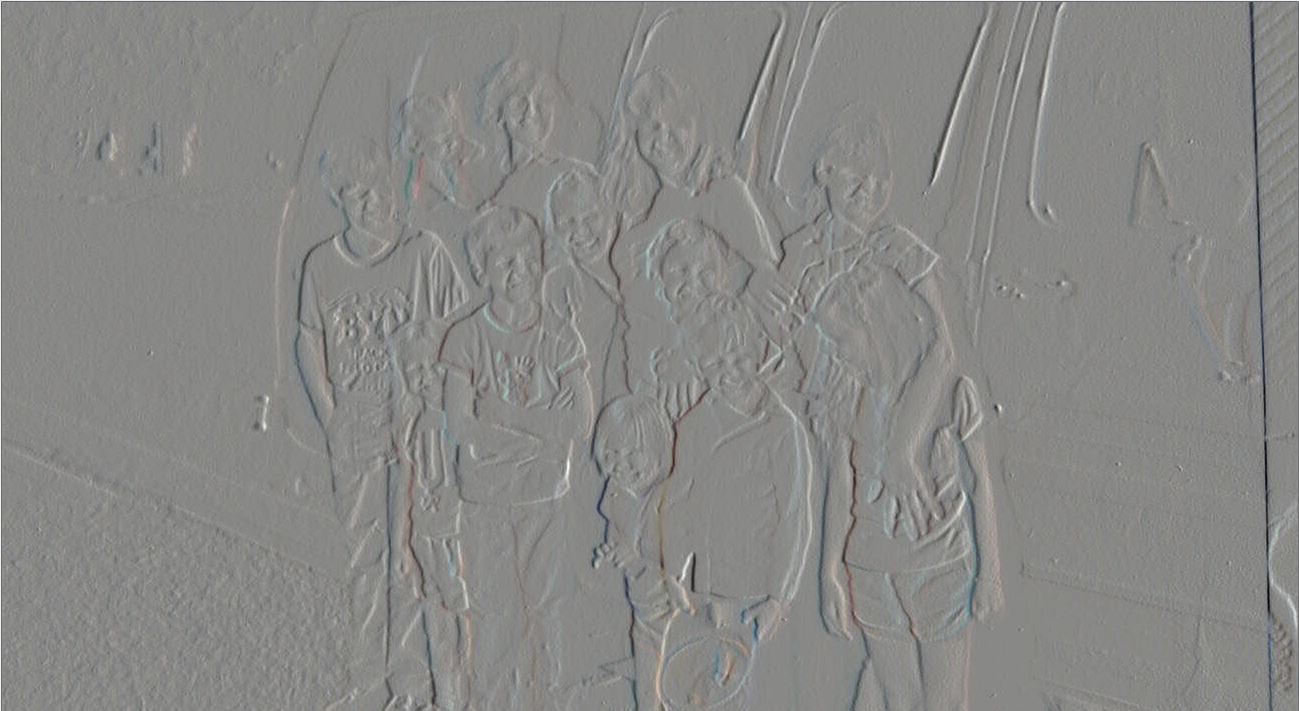
\includegraphics[width=.44\textwidth]{fig/gradientX.jpg}
\caption{\ensuremath{f_{x}}}
\label{ImageX}
\end{figure}

\begin{figure}
\centering
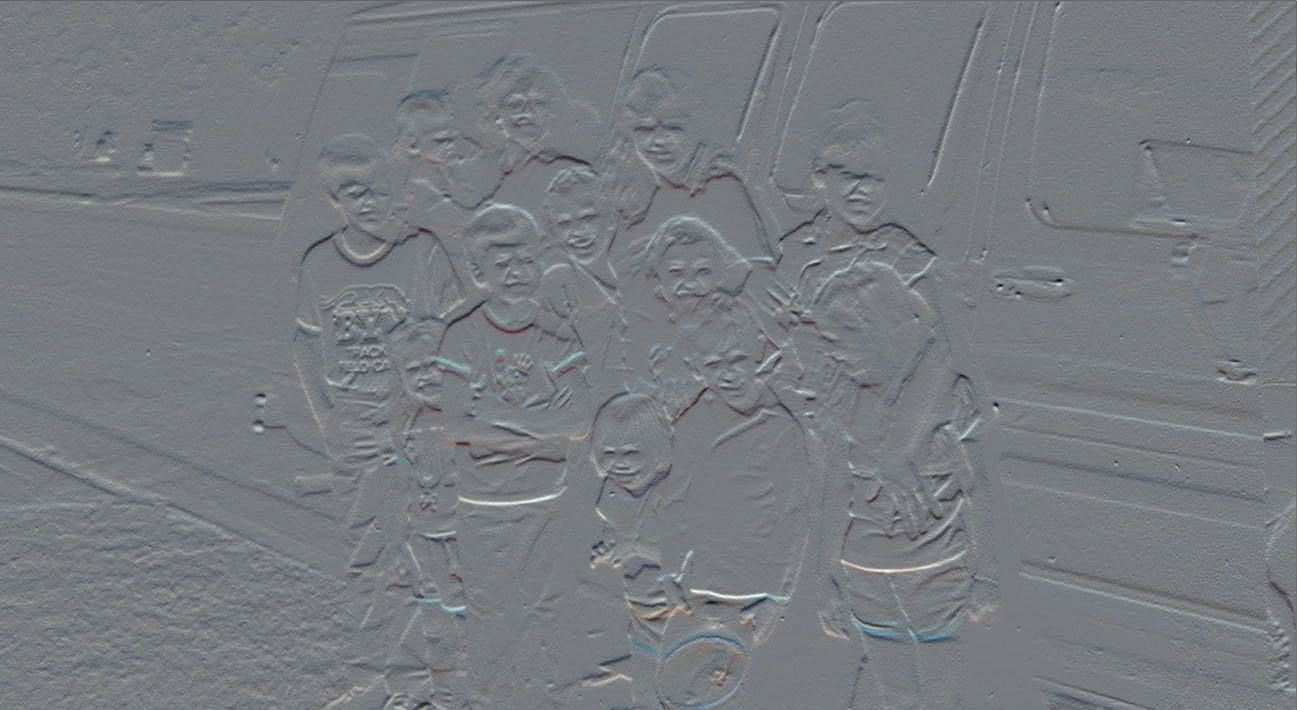
\includegraphics[width=.44\textwidth]{fig/gradientY.jpg}
\caption{\ensuremath{f_{y}}}   
\label{ImageY}
\end{figure}


\begin{figure}
\centering
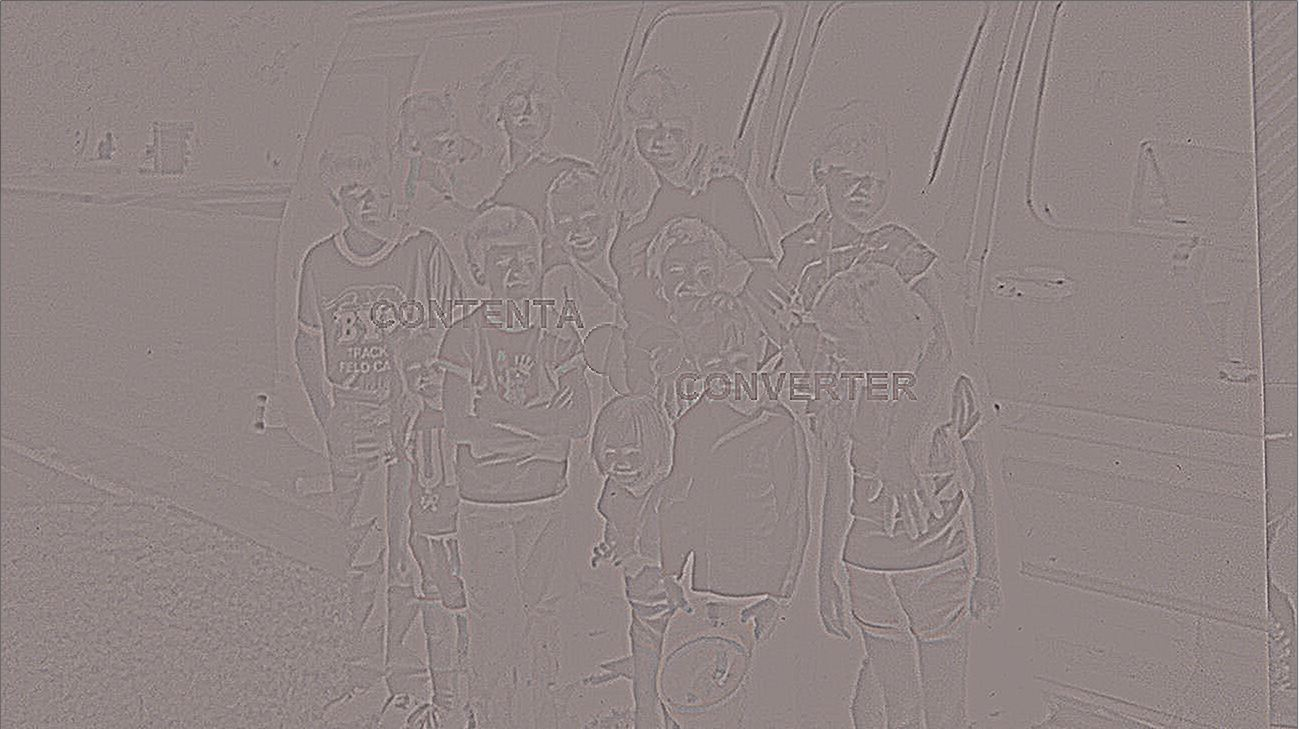
\includegraphics[width=.44\textwidth]{fig/divG.jpg}
\caption{\ensuremath{(f_{xx} + f_{yy})} The divergence of \ensuremath{f_{x}} and \ensuremath{f_{y}} normalized to display in an image.}
\label{div}
\end{figure}

The gradient field of our image can be shown with the scalar function previously explained. This is calculated by taking the difference between the current pixel and its neighbors. This is calculated with the follow equation, where \ensuremath{f_{x}} is the is the gradient in the x direction. The follow equations are used to calculate rate of change at every pixel. 

\begin{equation}
\ensuremath{f_{x}(i,j) = f(i)(j+1) - f(i)(j-1)}
\label{gradX}
\end{equation}

\begin{equation}
\ensuremath{f_{y}(i,j) = f(i+1)(j) - f(i-1)(j)}
\label{gradY}
\end{equation}

It is not possible to use these equations to calculate gradient at the border of an image.  The problem that occurs when using equations \ref{gradX} and \ref{gradY} is that these equations cannot be used to calculate the boundary conditions. If \ref{gradX} comes to a  boundary pixel it cannot use the equation calculate the gradient because there is no $j+1$ pixel. To overcome this boundary problem every boundary pixel is duplicated in both x and y axis. The duplicated pixels allow us to keep the original image size and still get the gradient of the image.

The divergence, which is the right hand side of Poisson's equation (\ref{poissonEqn}), can be calculated with the resulting gradient field of an image. An example of the divergence of figures \ref{ImageX} and \ref{ImageY} is seen in figure \ref{div}. The divergence is the second derivative of equations \ref{gradX} and \ref{gradY} added together:
\begin{equation}
\label{divergence}
div f = ( \frac{\delta^2 f}{\delta x^2} + \frac{\delta^2 f}{\delta y^2} ) = f_{xx}(i,j) + f_{yy}(i,j)
\end{equation}
The same boarder conditions apply to calculating divergence that happened with calculating the gradient. solve the boarder problem the same way we did for gradients and duplicate each border pixel.



Calculation of the gradient fields has resulting values between -255 and 255. But negative values cannot be represented in an image that has regular RGB values 0 to 255.  We normalize the gradient field array in order to display these values as an image in this paper. Following function is used to normalize the array:

\begin{equation}
\label{normalize}
\ensuremath{I(x,y) = \lfloor\frac{f(i,j) - f_{min}}{f_{max} - f_{min}} \times 255 \rfloor}
\end{equation}

\subsection{Poisson Solver}

In Poisson's equation discussed in section \ref{Poisson} there is one matrix \ensuremath{\Delta} and two vectors $f$, and div {\bf v}. The divergence vector {\bf v} is known by calculations from equation (\ref{div}), but there are two unknowns \ensuremath{\Delta} and $f$, which are respectivly the Laplacian, the image to be reconstructed. $f$ can be computed in a discrete way by expressing the Laplacian and divergence as discrete filters.  But this representation is difficult to solve for large vectors so an iterative Jacobi Poisson solver is used to approximate the solution. Using the Iterative Jacobi solver an image is regenerated from the divergence of that same image. 

To solve Poisson's equation (\ref{poissonEqn}) we express \ensuremath{\Delta} and the divergence as discrete filters. An example of a discretized Laplacian for a single pixel would use the following grid:
\begin{equation}
\label{lapDes}
\Delta \rightarrow  
\left[\begin{array}{ccc}
0 & -1 & 0 \\
-1 & 4 & -1 \\
0 & -1 & 0 \end{array}\right]
\end{equation}
The divergence of the image needs to be setup to be a single column matrix. To do this we stack the columns of the image on top of each other. The image to be reconstructed is also a vector of the same dimension as the divergence. The final representation of this equation for an image 4-by-4 pixels would look like Figure \ref{poissonGrid}. The resulting problem is reduced to a linear system but does not scale well as the image size increases, the size of the matrix also increases by factor $N^2$. 

\begin{figure}%[b]
\centering
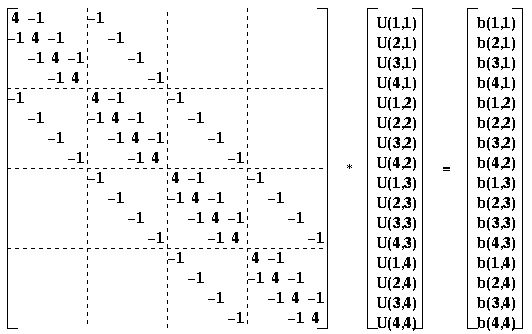
\includegraphics[width=.44\textwidth]{fig/matrix.jpg}
\caption{A 4-by-4 image setup as a discrete Poisson problem, image from \href{http://www.cs.berkeley.edu/~demmel/cs267/lecture24/lecture24.html}{Berkeley CS 267 class notes} }
\label{poissonGrid}
\end{figure}


{\bf Jacobi Method}
A Jacobi solver is used to approximate an image from the divergence, because direct solving of Poisson's equation (\ref{poissonEqn}) using the discretized Laplacian and divergence is not possible for large images. The algorithm for the Jacobi method is as follows:

\begin{tabbing}
initialize all of f'(x,y) to 0\\
do \= \\
\> for i to n \= \\
\>\> for j to m\=\\
\>  \> f(i,j) = (f'(i-1,j)+ f'(i+1,j)+ f'(i,j-1)+ f'(i,j+1)\\
\> \>      \>       + div(i,j))/4 \\
f'(i,j) = f(i,j)\\
while (image has not converged) \\
return f(i,j)
\end{tabbing}

This algorithm needs only one input which is the divergence {\bf v}. The algorithm initializes the approximation of the image to zero. Then the program goes to every pixel and takes its four neighbors and adds them and the {\bf div} of the pixel and then divides by four. This algorithm loops until the image converges or for a defined number of iterations. Our Jacobi approximation method minimizes the differences between $\nabla f$ and $div{\bf v}$.

{\bf Applying Mask} A Poisson solver create a transparent watermark on an image by adding the divergences of two images together. To do this we use two images, one that the original image and other has the watermark to be added. Both images are the same size and the watermark has a homogeneous background, except for the location of the watermark. The homogeneous background makes the divergence of the 0 every where except for the location of the watermark. Both images are added together and produce an image with a watermark.

\section{Artifacts}

We use the Jacobi method on a number of images and compare them to the original image. There are a few artifacts in the resulting image. The watermark functionality also can be improved. Our final images are computed with \iteration iterations of Jacobi method.

{\bf Regenerating image} Figure \ref{familyResult} is an example of running our implemention of the Jacobi method. This image compared to the the original fig \ref{family} has good coloring in the middle of the picture. One of the problems in the picture are that the boarders are white and do not have the same darker coloring of the original image. The artifacts occur due to our method of dealing with the boarder of the image, using the Jacobi method.

We tried two different methods when dealing with boarder pixels using the Jacobi method. The first method to deal with the board pixel was to not calculate that pixel and leave it at zero. The result of that method is shown in figure \ref{familyResult}. The other method we tried was similar to calculating the gradients. Boarder pixels were duplicated and instead of using adjacent non existing pixels the duplicated pixel was used. The result of that method is figure \ref{familyBoarder}, it produced an image that was much darker than the original image. The original method of calculating boarder pixels, which left boarder pixels at zero, while the Jacobi method was calculated is used for all images in this paper.

{\bf Watermark} An example of the watermark feature of our application is figure \ref{mask}. The image produced by the watermark has more artifacts than only regenerating the image. Simply adding divergence of the watermark and the image sometimes caused the image to not have equal levels over the entire image. One way to fix this may be to use only a small ratio of the divergence of the watermark. We did when the divergence of the watermark was small it would allow the image to produce a result much closer to that seen in when only regenerating an image.

\section{Future Work}



Poisson's equation allows regeneration of images that have changed gradient fields, or seamlessly integration of two images as discussed in section \ref{relatedWork}. Watermark feature of the project produces initial results on seamless integration of images, and is to how drag and dropping discussed by \cite{ddp} works. Further work includes adding boundary calculations to improve the boarder of the image that is being pasted on. Adding or removing the transparency of an integrated image can also help improve the final image. 

Further exploration is necessary to implement an image restoration feature to this project. In order to accomplish this divergences need to be estimated for the mission sections of an image, and is discussed by \cite{Perez}. A mask may be used to identify what parts of the image needs restoration. With the mask estimations of missing sections are calculated and an linear solver can reproduce an image to restore missing, or damaged sections. 

\begin{figure}
\centering
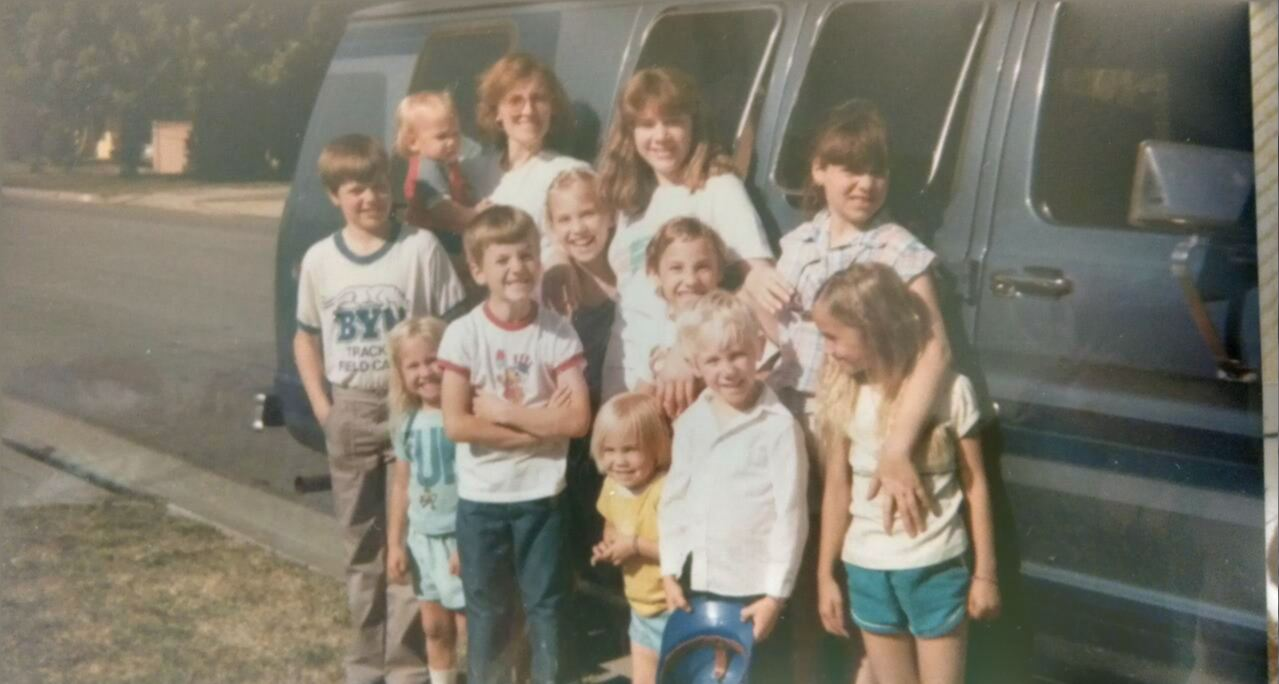
\includegraphics[width=.44\textwidth]{fig/familyResult.jpg}
\caption{An approximation using Jacobi method to solve for the original image. With boarder pixels ignored.}
\label{familyResult}
\end{figure}

\begin{figure}
\centering
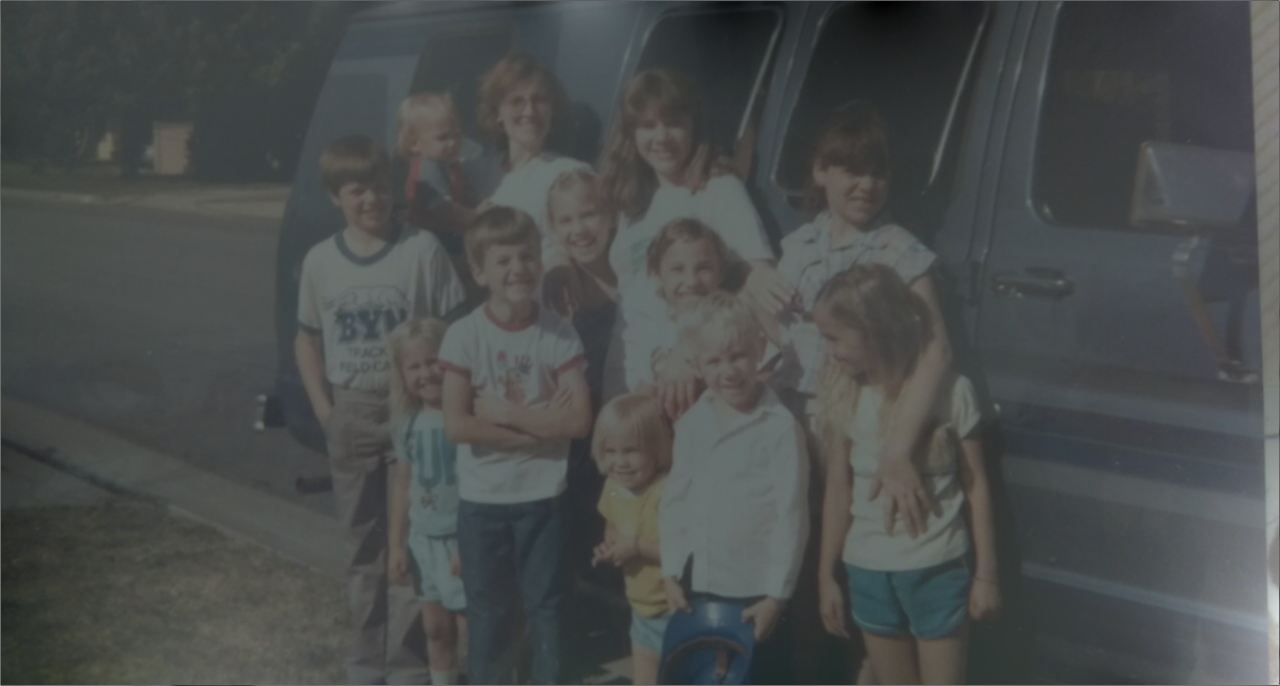
\includegraphics[width=.44\textwidth]{fig/familyBoarder.jpg}
\caption{An approximation using Jacobi method to solve for the original image. With boarder pixels duplicated.}
\label{familyBoarder}
\end{figure}

\begin{figure}
\centering
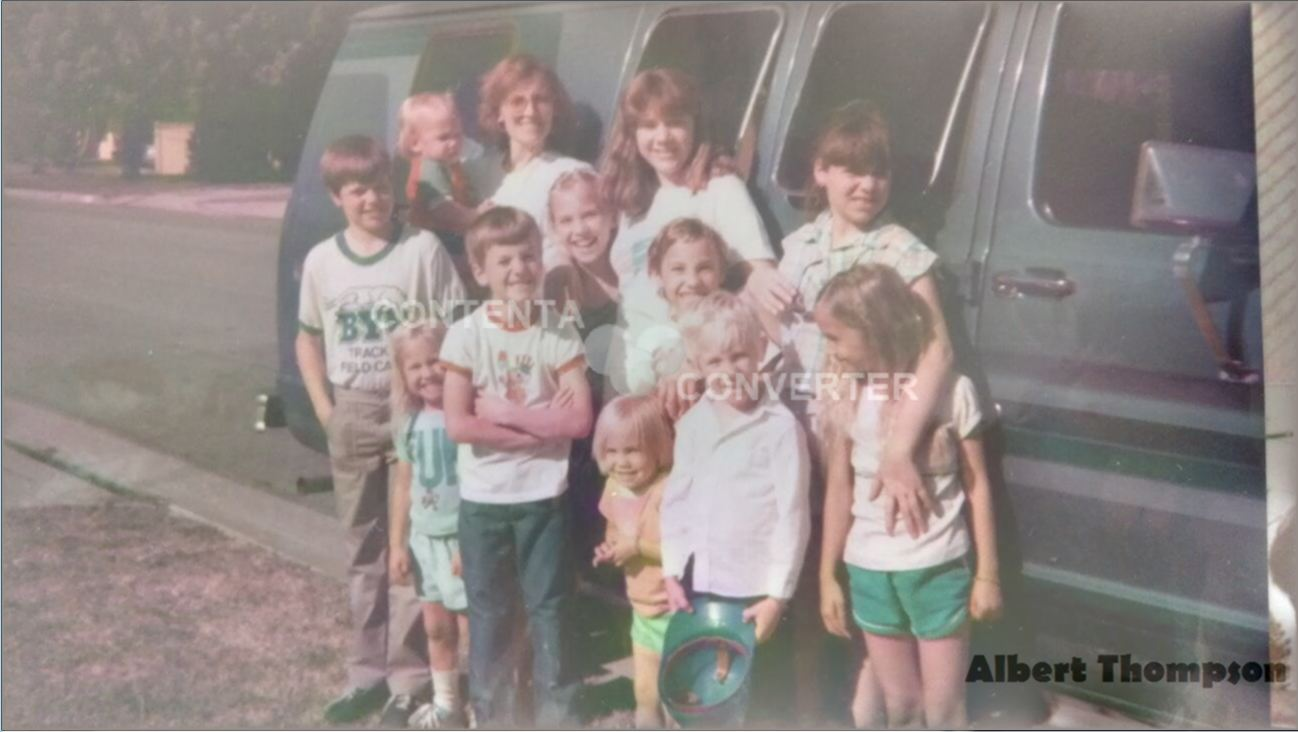
\includegraphics[width=.44\textwidth]{fig/mask.jpg}
\caption{An example watermark on an image.}
\label{mask}
\end{figure}

There are many different methods that can compute the linear equation (\ref{poissonEqn}) and minimize the difference in the original image and desired image. The Jacobi method used solve Poisson's equation is slow. A different linear solver can be implemented to improve the speed of the program. The Jacobi method in calculates linear problems in $N^2$ time. An improvement to the project would be to use the the conjugate gradient implementation which cuts the calculation time to $N^(3/2)$, or Fast Fourier Transform calculates in only $N$ time. Further research allows us to change from using the Jacobi method and implement other linear solvers.

\section{Conclusion}

We show how Poisson's equation is used to regenerate an image from the divergence of gradient fields. We calculate gradients of an image and also take in to account the boarder conditions. An implementation of the Jacobi method solves Poisson's equation using only a divergence. Our program obtains images that looked similar to our original image.

The Jacobi method provided us with an initial experience on methods of solving Poisson's equation. An implementation of a water mark feature demonstrates how image divergences can be layer to produce a new image. Implementing our watermark method allowed us to see how images react when two divergences are added together. Further work includes implementing further gradient manipulations and refining our calculation of boundary conditions.


\begin{figure}[b]
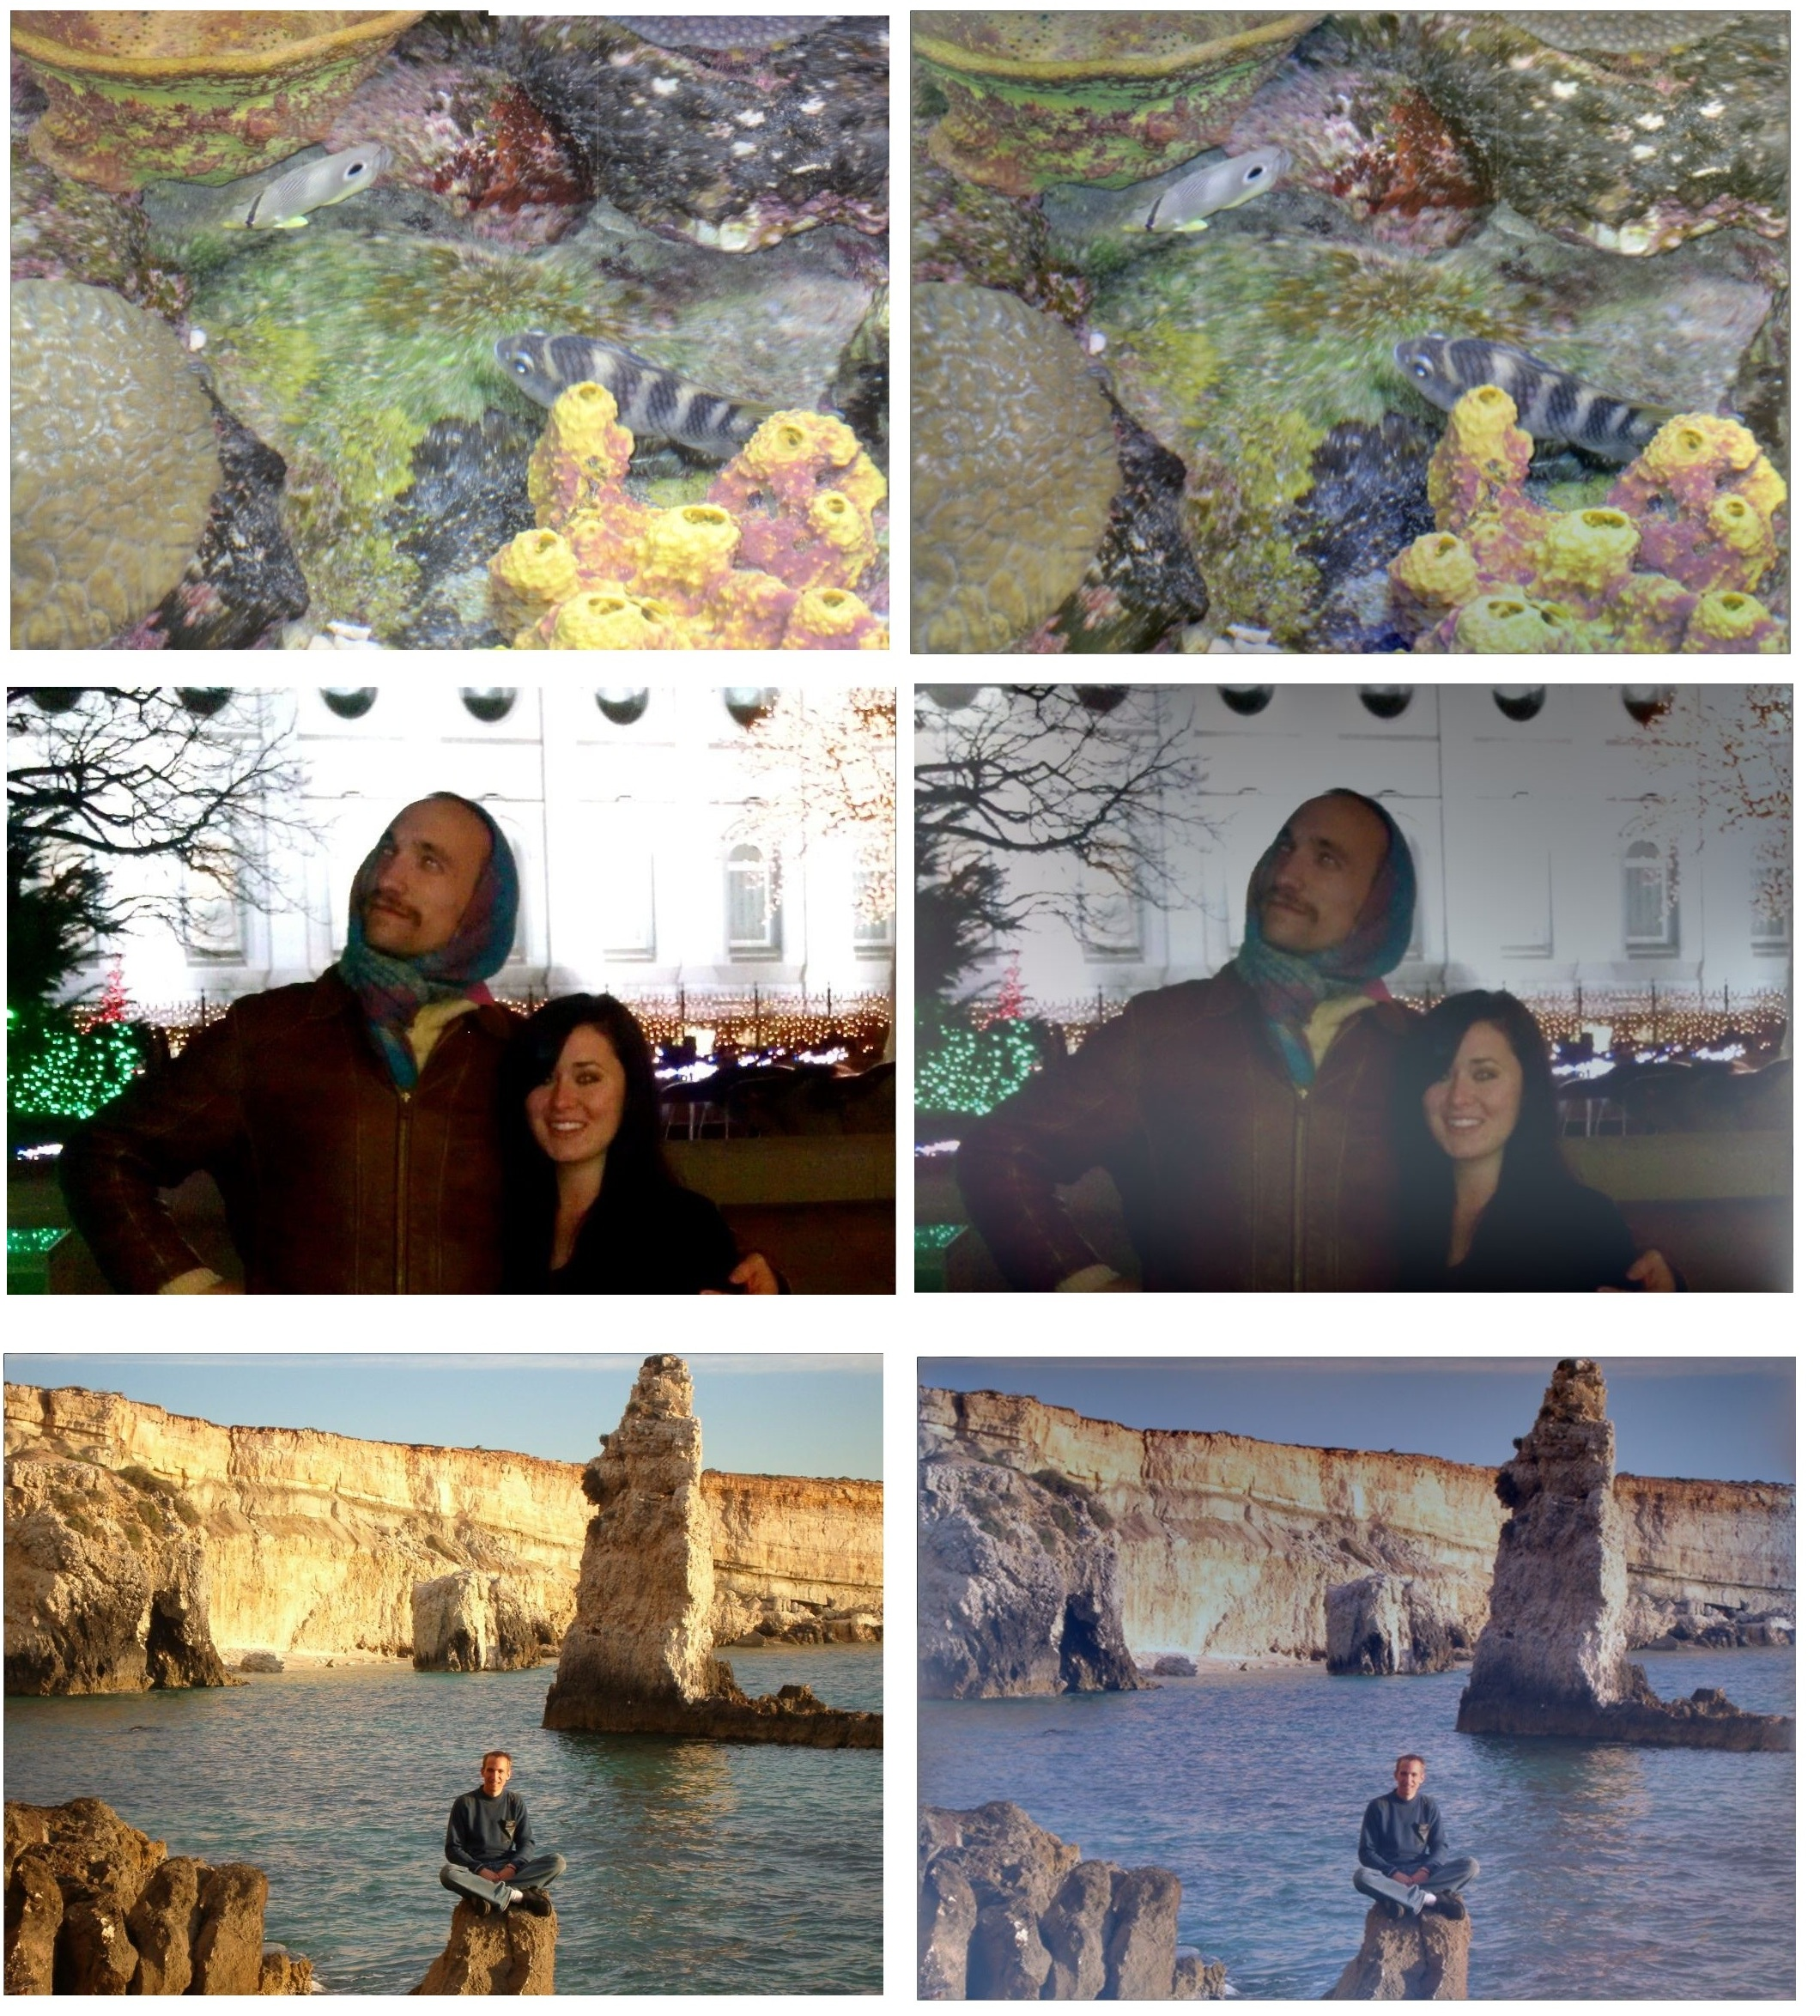
\includegraphics[width=\linewidth]{fig/compilation.jpg}
\caption{The right column is a the set of original photos the left columb is a set of generated photos}
\label{mask}
\end{figure}


\bibliographystyle{acmsiggraph}
{\small\bibliography{bibliography}}

%%%%%%%%%%%
%
% Do not change anything below this line!!!
%
%%%%%%%%%%%


% adds an empty page to documents with odd page number. This is to
% make sure that the first page of every paper starts at an odd page.
\cleardoublepage

\end{document}

% LocalWords:  CPSC Heidrich PDF cpsc tex dvi xdvi BibTeX bibtex PostScript ps
% LocalWords:  dvips Ppdf pdf pdflatex EPS PNG includegraphics
